% *********************************************************************
% © 2026 Jeremy Sylvestre
%
% Permission is granted to copy, distribute and/or modify this document
% under the terms of the GNU Free Documentation License, Version 1.3 or
% any later version published by the Free Software Foundation; with no
% Invariant Sections, no Front-Cover Texts, and no Back-Cover Texts. A
% copy of the license is included in the appendix entitled “GNU Free
% Documentation License” that appears in the output document of this
% PreTeXt source code. All trademarks™ are the registered® marks of
% their respective owners.
%
% *********************************************************************
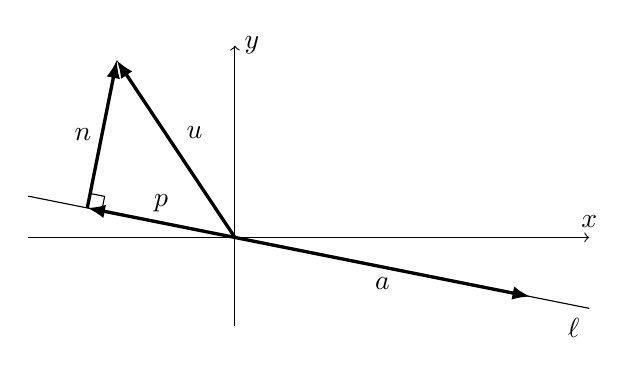
\begin{tikzpicture}[
	vector/.style={-latex,very thick},
	scale=0.75
]
	\coordinate (o) at (0,0);
	\coordinate (u) at (-2,3);
	\coordinate (a) at (5,-1);
	\coordinate (p) at (-2.5,0.5);

	\draw[->] (-3.5,0) to (6,0) node[above] {$x$};
	\draw[->] (0,-1.5) to (0,3.25) node[right] {$y$};

	% parallel to (5,-1)
	\draw[thin] (-3.5,0.7) to (6,-1.2) node[below left] {$\ell$};

	\draw[vector] (o) to node[above right] {$\uvec{u}$} (u);
	\draw[vector] (o) to node[below] {$\uvec{a}$} (a);
	\draw[vector] (o) to node[above] {$\uvec{p}$} (p);
	\draw[vector] (p) to node[left] {$\uvec{n}$} (u);

	% perp symbol
	\begin{scope}[xshift=-2.5cm,yshift=0.5cm]
		\draw[thin,rotate=-11.31] (0.25,0) to (0.25,0.25) to (0,0.25);
	\end{scope}

\end{tikzpicture}
